\section{Uczenie sieci neuronowej}
\subsection{Architektura algorytmu wykrywającego obiekty} \label{section:architekturaAlgorytmu}
Do zbudowania modelu wykrywającego wskazane klasy na zdjęciach użyto oprogramowania Matlab, dodatku
Deep Learning Toolbox oraz innych dodatków pozwalających na przetwarzanie obrazu. 
Wykorzystany model bazuje na sieci neuronowej nazwanej CSPDarkNet53 i wstępnie wytrenowanym na 
zbiorze \href{https://cocodataset.org/}{COCO} zawierającym ponad 200 tysięcy oznaczonych zdjęć i 80 różnych kategorii.
\begin{figure}[H]
	\centering
	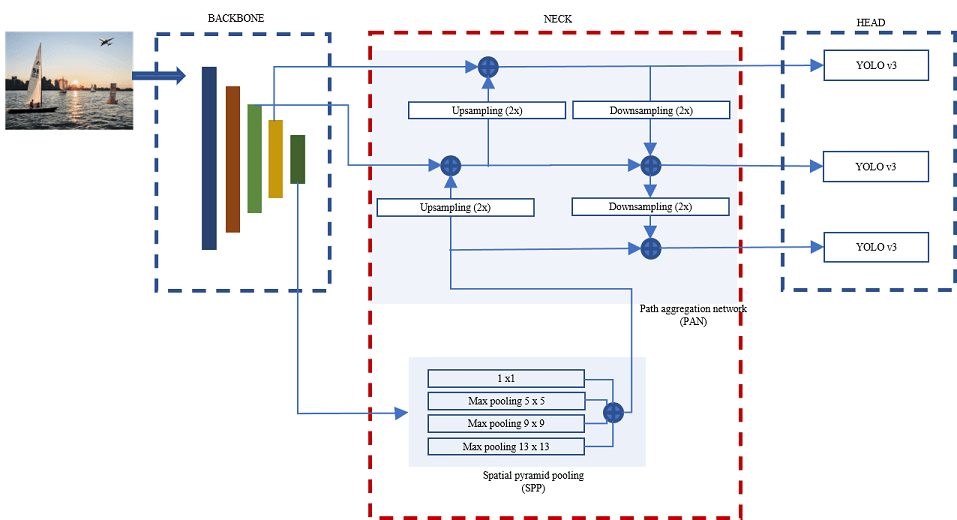
\includegraphics[width=12cm]{pages/uczenie/img/yolov4architecture.png}
	\caption{Sposób implementacji modelu YOLOv4 w Matlab'ie \cite{matlabOYolov4}}
	\label{fig:implementacjaWMatlabie}
\end{figure}
Implementacja algorytmu YOLO w Matlabie została podzielona na trzy różne sekcje. 
Pierwsza, oznaczona na rysunku \ref{fig:implementacjaWMatlabie} jako 'backbone', jest szkieletem sieci odpowiadającym za obliczenie 
mapy cech z obrazów wejściowych. Druga warstwa, łączy mapy cech z danymi z warstw sieci szkieletowej oraz wysyła je do kolejnego modułu.
Ostatni segment odpowiada za przetworzenie wcześniej wyodrębnionych cech, przewidzenie obwiedni i klasy obiektów.
\begin{figure}[H]
	\centering
	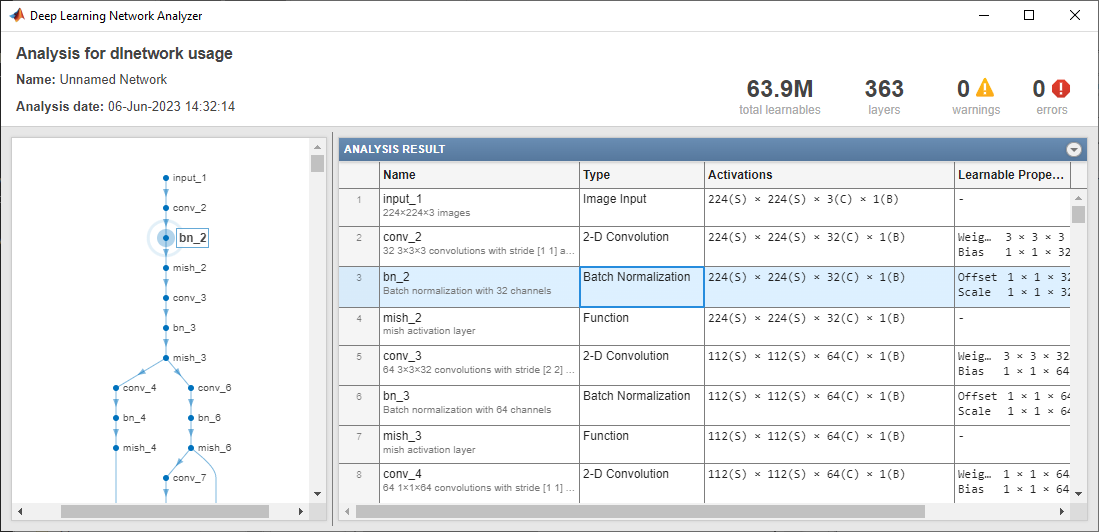
\includegraphics[width=10cm]{pages/uczenie/img/wielkoscSieciMatlabAnalyze.png}
	\caption{Parametry użytej sieci uzyskane funkcją analyzeNetwork}
\end{figure}

Użyta sieć składa się z 53 warstw konwolucyjnych, wejścia 224x224x3 oraz trzech 
wyjść określających prawdopodobieństwo występowania danej klasy. 
Cała sieć zbudowana jest z 363 warstw a do wyuczenia jest ponad 63mln parametrów.

Istnieje mniejsza sieć nazwana 'Tiny-YOLOv4', która posiada zaledwie około 30 warstw konwolucyjnych, dzięki czemu
została znacznie zwiększona szybkość działania, kosztem niewielkiego pomniejszenia skuteczności. 
Według wielu różnych źródeł wersja ta jest zdecydowanie lepsza do przetwarzania szybko zmieniającego się obrazu.
%========================================================
\subsection{Zbieranie danych}
\subsubsection{Automatyczne generowanie danych}
W pierwszej wersji dane miały być generowane przy pomocy automatycznego skryptu.
Utworzony program w Matlabie, otwierał wcześniej nagrany film z samym tłem, a następnie 
na pobranych klatkach obrazu wstawiał szablony z przygotowanymi obrazami docelowych obiektów.
Dzięki dynamicznemu generowaniu, można było zachować zróżnicowanie danych pomimo ich dużej ilości.

\begin{figure}[H]
	\centering
	\begin{minipage}{0.45\textwidth}
		\centering
		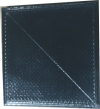
\includegraphics[width=3.5cm]{pages/uczenie/img/maska_kw3.png}
	\end{minipage}
	\begin{minipage}{0.45\textwidth}
		\centering
		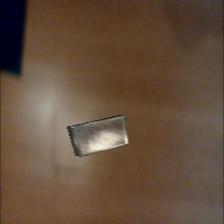
\includegraphics[width=3.5cm]{pages/uczenie/img/wynikGenerowania.jpg} % second figure itself
	\end{minipage}
	\caption{Lewe zdjęcie przedstawia maskę z usuniętym tłem a prawe klatkę nagranego filmu z naniesionym obiektem}
	\label{rys:przykladoweGenerowanieDanych}
\end{figure}

Jak widać na rysunku \ref{rys:przykladoweGenerowanieDanych}, generowane dane wyglądają dosyć sztucznie, głównie ze względu na 
tło oraz niekonsekwentne oświetlenie obiektu i tła. Ostatecznie wynikiem działania algorytmu był utworzony zbiór zdjęć
oraz jeden plik typu gTruth z zapisanymi obrazami, lokalizacją i klasą obiektów.
Poniżej dołączono skróconą wersje programu generującego zdjęcia.

\begin{lstlisting}[language=Matlab,caption=Generowanie danych]
	% automatyczne generowanie danych do uczenia sieci
	clc; clear;  close all;
	
	videoFiles = ["data/vid/w1.3gp", "data/vid/w2.3gp"];
	pathToSaveImages = "data/test2";
	outputImageSize = [224, 224];
	filterToOutputImage = fspecial("motion", 2, 2);
	
	dataKolo = {}; dataKwadrat = {}; dataTrojkat = {};
	dataFileNames = "";
	for vidName = videoFiles
		vid = VideoReader(vidName); %wczytanie filmu
		rrStep = int8(vid.NumFrames);
		for fIndX = 1 : 5 : vid.NumFrames % iteracja po klatkach
			frame = read(vid, fIndX);
	
			% dostosowanie klatki do rozmiaru sieci
			frame = imresize(frame, outputImageSize);
	
			% losowanie odpowiedniej maski/obiektu
			rr = randi([1, 6]);
			if(rr == 1) 
				[x, map, alpha] = imread("data\mask\kw_mask.png");
			% wczytywanie kolejnych masek
			end
			x = imresize(x, 0.5);
			alpha = imresize(alpha, 0.5);
			maskSize = size(x);        
			%wyznczenie pozycji 
			posX = randi([0, outputImageSize(1) - maskSize(1)]);
			posY = randi([0, outputImageSize(2) - maskSize(2)]);
	
			if(rr == 1 || rr == 2) % kwadrat
				dataKolo(end + 1) = {[]};
				dataKwadrat(end + 1) = {[posX, posY, maskSize(1), maskSize(2)]};
				dataTrojkat(end + 1) = {[]};
			elseif (rr == 5 || rr == 6 || rr > 5) % kolo
				dataKolo(end + 1) = {[posX, posY, maskSize(1), maskSize(2)]};
				dataKwadrat(end + 1) = {[]};
				dataTrojkat(end + 1) = {[]};
			elseif (rr == 3 || rr == 4) % tr
				dataKolo(end + 1) = {[]};
				dataKwadrat(end + 1) = {[]};
				dataTrojkat(end + 1) = {[posX, posY, maskSize(1), maskSize(2)]};
			end
	
			if (fIndX > rr * rrStep)
				rr = rr + 1;
			end
	
			% wzstawienie szablonu do obrazu
			frame = insertImageInPos(frame, x, alpha, posX, posY);
			% dodanie opcjonalnego filtru do zdjecia 
			if exist("filterToOutputImage" ,"var") == true
				frame = imfilter(frame, filterToOutputImage);
			end
	
			path = sprintf("%s/%i-%i.jpg", pathToSaveImages,randi(300), fIndX);
			dataFileNames = dataFileNames + path + ";";

			%zapisanie obrazu
			imwrite(frame, path)
		end
	end
	
	% zapisywanie danych jako obiektu datastore
	labels = labelDefinitionCreator();
	addLabel(labels, "kolo", "Rectangle");
	addLabel(labels, "kwadrat", "Rectangle");
	addLabel(labels, "trojkat", "Rectangle");
	labelData = table(dataKolo', dataKwadrat', dataTrojkat', 'VariableNames',{'kolo', 'kwadrat', 'trojkat'});
	
	t = split(dataFileNames, ";"); t(end) = [];
	f =  matlab.io.datastore.FileSet(t);
	imds = imageDatastore(f);
	labelDataStore = boxLabelDatastore(labelData);
	ds = combine(imds, labelDataStore);
	save("ds", "ds");
\end{lstlisting}
Skrypt otwierał wskazany film i pobierał co 5 klatkę obrazu. Dalej generowana była liczba określająca klasę wstawionego obiektu.
Szablon był wczytywany do pliku, a typ i losowo wygenerowana pozycja została zapisana w bazie danych.
Na końcu mógł zostać dodany filtr, mający poprawić efekt przejścia pomiędzy połączonymi obrazami. 
Tak przygotowane zdjęcie zostało zapisane na dysku. 
Po przetworzeniu filmu dane o obiektach, ich pozycjach oraz odpowiednich zdjęciach były zapisywane do odpowiedniego pliku.
\begin{figure}[H]
	\centering
	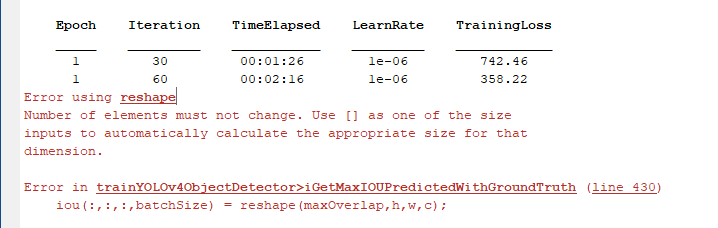
\includegraphics[width=12cm]{pages/uczenie/img/errorPrzyTrenowaniu.png}
	\caption{Błąd podczas trenowania obrazu}
\end{figure}
Ostatecznie największym problemem okazało się wytrenowanie sieci na tak wygenerowanych danych.
Prawdopodobnie algorytm źle zapisywał dane, ponieważ w trakcie trenowania pierwszej epoki i losowej iteracji trenowanie przerywało się,
wyświetlając komunikat z błędem funkcji 'reshape' wywoływanej wewnątrz funkcji trenującej model.

\subsubsection{Ręczne oznaczanie danych}
Docelowa i działająca sieć została wytrenowana na ręcznie oznaczonych zdjęciach. 
Dane zostały zebrane na wykonanym już robocie i nagrane poprzez symulowanie ruchów robota i przesuwanie docelowych obiektów.
Nagrane filmy zostały przetworzone poprzez skrypt, który pobrał z filmu co którąś klatkę a następnie przeskalował ją do docelowego rozmiaru. 


\begin{figure}[H]
	\centering
	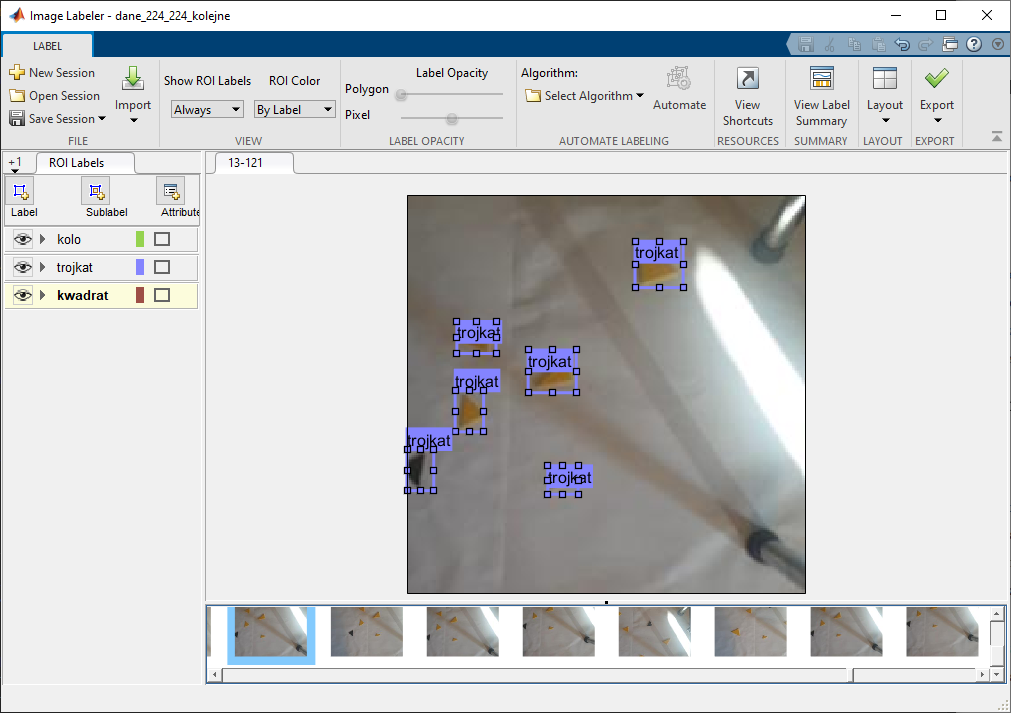
\includegraphics[width=12cm]{pages/uczenie/img/imageLabeler.png}
	\caption{Program imageLabeler, pozwalający na etykietowanie zdjęć}
	\label{fig:imgageLabelerMatlab}
\end{figure}
Rysunek \ref{fig:imgageLabelerMatlab} przedstawia zrzut ekranu programu, w którym zdefiniowano odpowiednie klasy, wczytano 
przygotowane dane oraz oznaczono odpowiednie obiekty ich klasami.
Baza zawiera ponad 1200 zdjęć z obiektami (zmienione orientacje, pozycje, kształt) i różnym tłem (zmiana oświetlenia, dodatkowe cienie).

\begin{figure}[H]
	\centering
	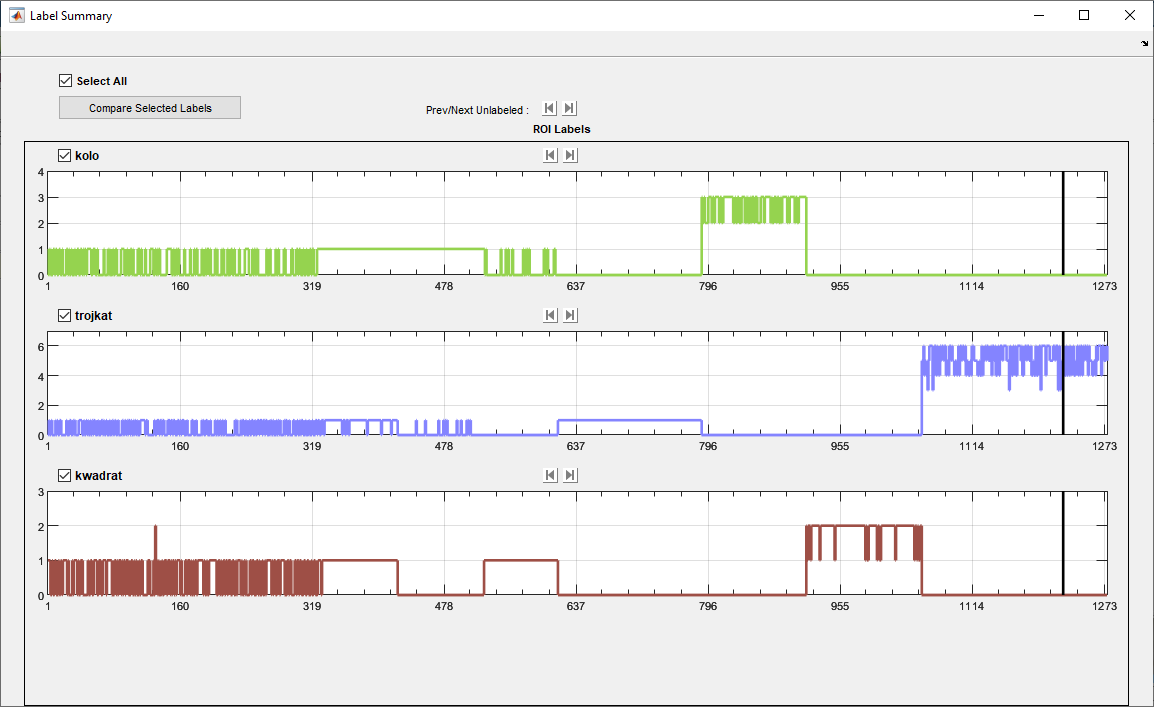
\includegraphics[width=14cm]{pages/uczenie/img/podsumowanieRozkladuEtykiet.png}
	\caption{Rozkład klas w poszczególnych zdjęciach}
\end{figure}
Baza zdjęć była systematycznie zwiększana wraz z analizą skuteczności działania wytrenowanej sieci. 
Jak widać najwięcej jest zdjęć zawierających kwadraty, a najmniej, ze względu na uniwersalny kształt, kół. 
Ostatecznie rozkład klas prezentuje się następująco: 
\begin{figure}[H]
	\centering
	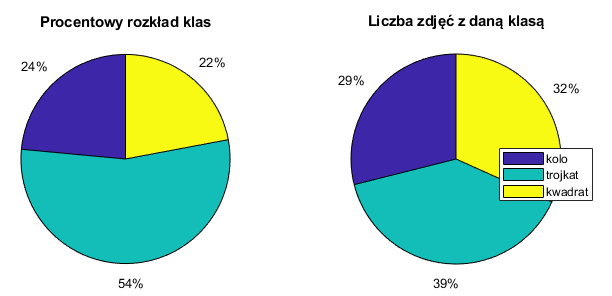
\includegraphics[width=16cm]{pages/uczenie/img/rozkladKlas.png}
	\caption{Ogólny rozkład klas}
\end{figure}
Jak widać zgodnie z oczekiwaniami w bazie ze względu na największą ilość konfiguracji jest najwięcej zdjęć trójkątów. 
Liczba kół i kwadratów jest bardzo podobna. 
Poniżej został zaprezentowane przykładowe zdjęcia. 
\begin{figure}[H]
	\centering
	\begin{minipage}{0.30\textwidth}
		\centering
		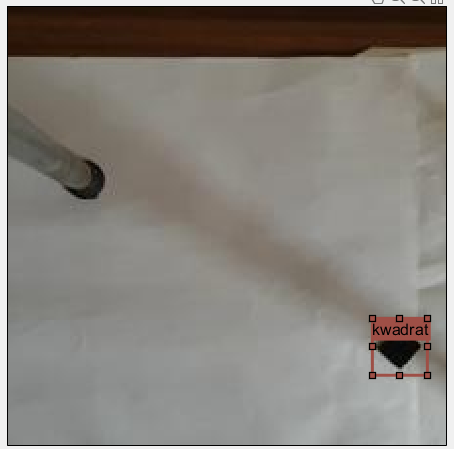
\includegraphics[width=4.5cm]{pages/uczenie/img/przykladoweDaneV1.png} % first figure itself
	\end{minipage}\hfill
	\begin{minipage}{0.3\textwidth}
		\centering
		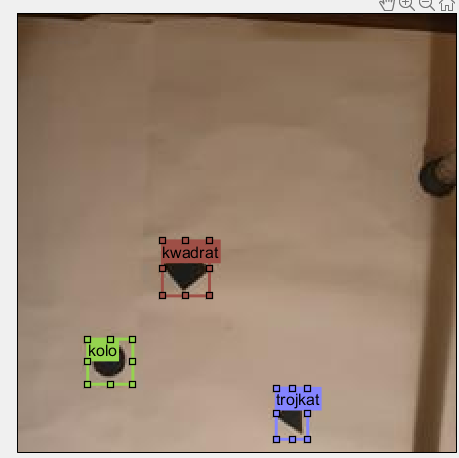
\includegraphics[width=4.5cm]{pages/uczenie/img/przykladoweDaneV2.png} % second figure itself
	\end{minipage}\hfill
	\begin{minipage}{0.3\textwidth}
		\centering
		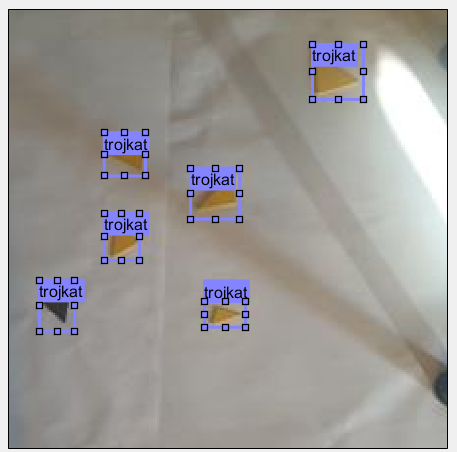
\includegraphics[width=4.5cm]{pages/uczenie/img/przykladoweDaneV3.png} % second figure itself
	\end{minipage}
						
	\caption{Przykładowe otagowane zdjęcia}
\end{figure}
Pierwsze fotografie zawierają pojedyncze obiekty, jednak wraz z rozwojem, na zdjęciach pojawiało się coraz więcej różnych obiektów.
%========================================================
\subsection{Uczenie sieci}
Sieć neuronowa była trenowana przy pomocy toolbox'a Deep Learning Toolbox w Matlabie, przy pomocy poniższego skryptu.
% \begin{lstlisting}[language=Matlab,caption=Uczenie sieci]

% \end{lstlisting}
\lstinputlisting[language=Matlab,caption=Uczenie sieci]{pages/uczenie/skryptUczenie.txt}


Ze względu na małą ilość pamięci graficznej, uczenie odbywa się na procesorze. 
Podczas jednej iteracji, algorytm przetwarza jednocześnie 16 zdjęć (parametr MiniBatchSize). Przy takiej konfiguracji, uczenie 
na GPU nie było możliwe, a jednocześnie po zmniejszeniu tego parametru do 1 uczenie nie było tak skuteczne jak w przypadku jednoczesnego 
przetwarzania większej ilości obrazów.
Parametry uczenia sieci:
\begin{itemize}
	\item metoda uczenia: sgdm (Stochastic Gradient Descent with momentum),
	\item współczynnik uczenia: 0.001,
	\item liczba epok: 20.
\end{itemize}
Ostatecznie finalny model był douczany przy pomocy powyższego skryptu trzy razy co oznacza, że przeszedł przez 60 epok. 
Zbyt duża ilość epok uczących sieć może spowodować negatywny wynik z powodu przetrenowania sieci i ścisłego dopasowania się do danych treningowych.
\begin{figure}[H]
	\centering
	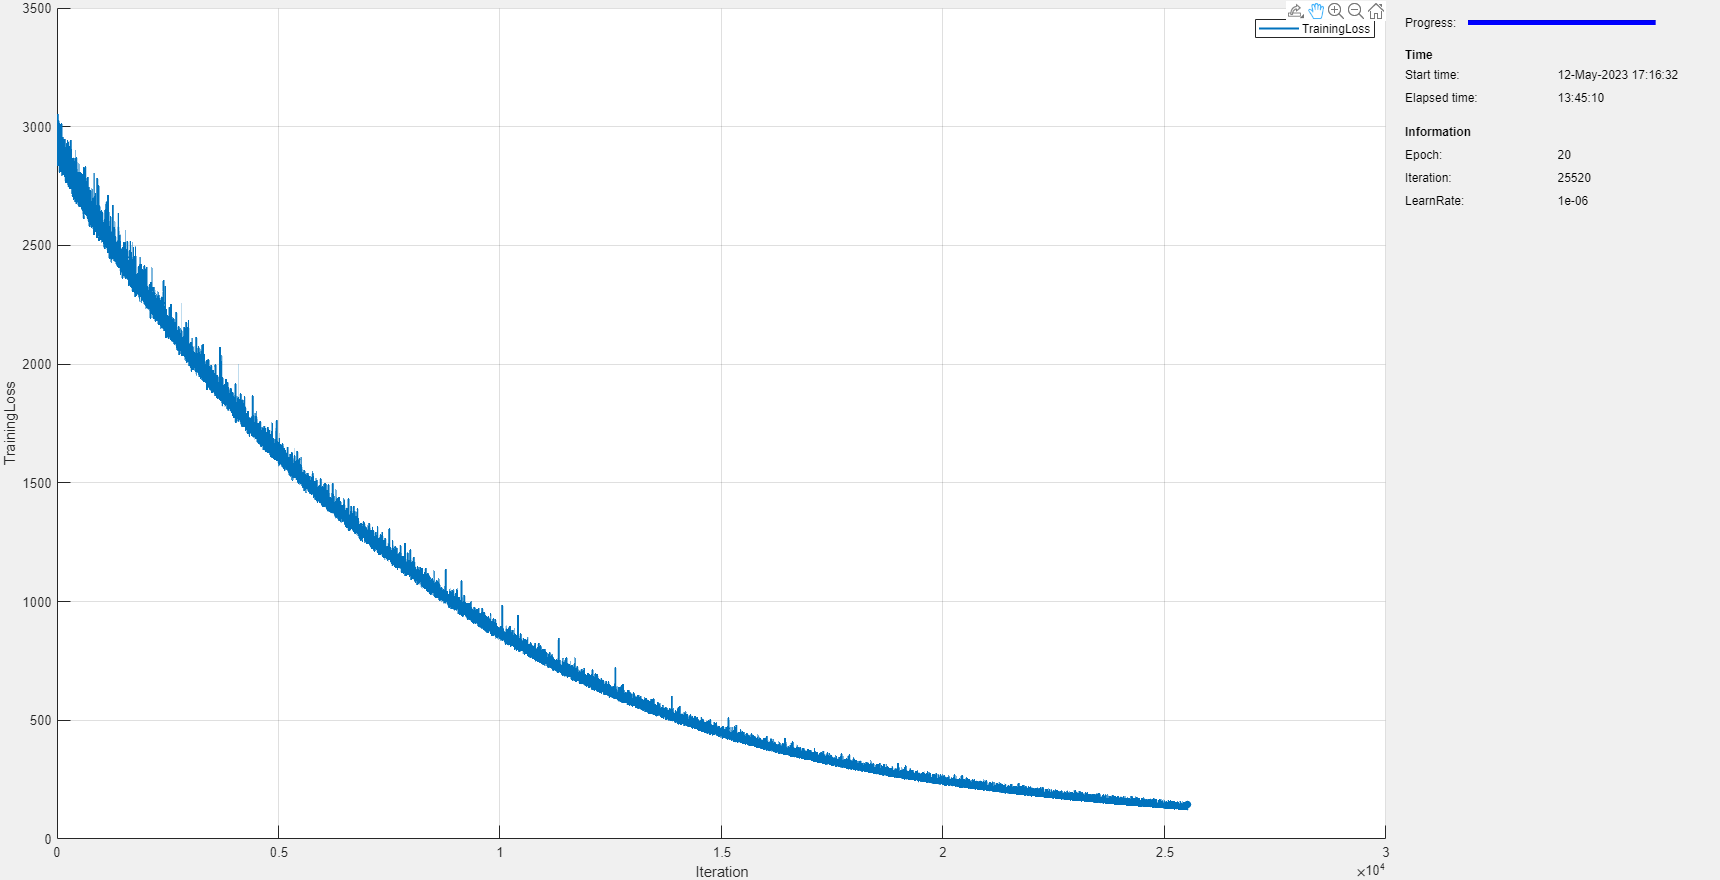
\includegraphics[width=14cm]{pages/uczenie/img/wykresTrenowanie.png}
	\caption{Przebieg błędu w zależności od liczby epok}
	\label{fig:bladWUczeniu}
\end{figure}
Wykres z rysunku \ref{fig:bladWUczeniu}, przedstawia przebieg trenowania i spadku błędu. Widać, że na początku procesu błąd bardzo szybko spada, 
jednak od połowy uczenia tendencja spada. Zdjęcie pochodzi z pierwszego etapu trenowania, gdzie trenowanie było efektywniejsze. 
Kolejne dwa etapy trenowania cechowały się spadkiem z około 50 do 0,2 wartości błędu. 

\subsection{Testy}
Aby sprawdzić skuteczność sieci, przeprowadzono testy polegające na podaniu wcześniej
niewidzianego obrazu z wieloma obiektami, 
ręczne przeanalizowanie wyników sieci i porównanie ich z rzeczywistą liczbą obiektów.
\begin{figure}[H]
	\centering
	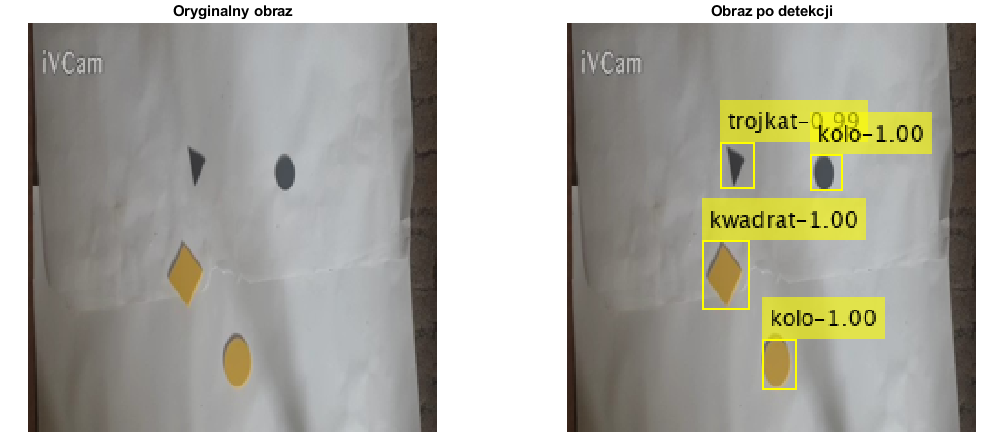
\includegraphics[width=15cm]{pages/uczenie/img/testyWynikSieci1.png}
	\caption{Pierwszy test z dobrym oświetleniem}
	\label{fig:testSieci1}
\end{figure}
Na podstawie wyniku pokazanemu na rysunku \ref{fig:testSieci1} widać, że sieć w sprzyjających warunkach radzi sobie z rozpoznawaniem różnych obiektów,
leżących w różnych orientacjach i pozycjach. Równocześnie należy zwrócić uwagę na bardzo duże wskaźniki pewności sieci wykrytych obiektów. 
\begin{figure}[H]
	\centering
	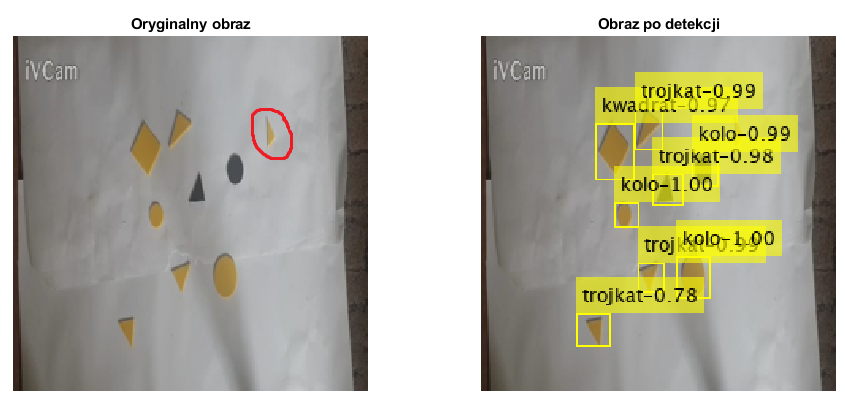
\includegraphics[width=15cm]{pages/uczenie/img/testyWynikSieci2.png}
	\caption{Test z dużą ilością różnych obiektów}
	\label{fig:testSieci2}
\end{figure}
Analizując przypadek przy dobrym oświetleniu z rysunku \ref{fig:testSieci2}, widać, że sieć ogólnie dobrze poradziła sobie z tak dużą liczbą różnych obiektów. 
Analizując dokładniej obraz, można zauważyć, że nie wykryty został jeden mniejszy trójkąt (zaznaczony na czerwono).
\begin{figure}[H]
	\centering
	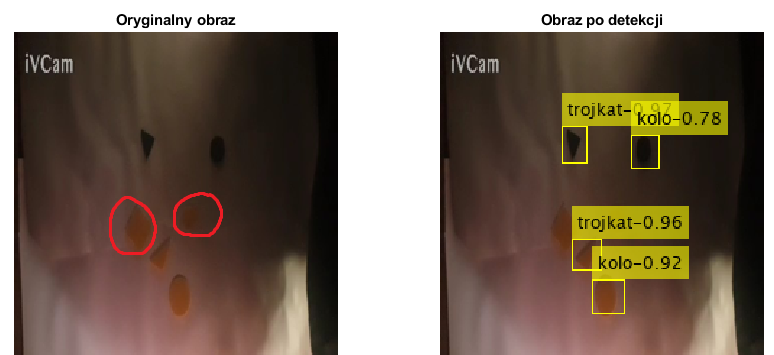
\includegraphics[width=15cm]{pages/uczenie/img/testyWynikSieci3SlabeOsw.png}
	\caption{Test przy słabym oświetleniu}
	\label{fig:testSieci3}
\end{figure}
Po ograniczeniu światła sieć rozpoznała tylko cztery z sześciu obiektów. 
Równocześnie w porównaniu do poprzednich eksperymentów spadły wskaźniki pewności.
Należy zauważyć, że pominięte obiekty są bardzo słabo widoczne i w pierwszej chwili
nawet ludzkie oko może mieć problem z szybką lokalizacją.
\begin{figure}[H]
	\centering
	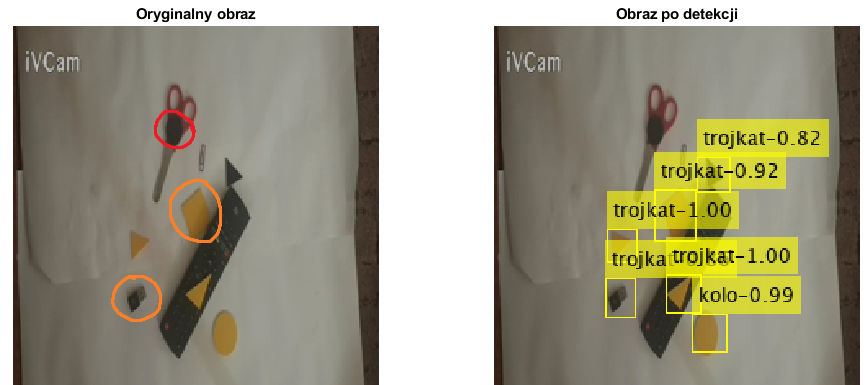
\includegraphics[width=15cm]{pages/uczenie/img/testyWynikSieci4.png}
	\caption{Testy z nieznanymi obiektami}
\end{figure}
Ostatni test został przeprowadzony po dodaniu nieznanych sieci obiektów.
Widać, że sieć nie rozpoznała leżącego na nożyczkach koła i 
źle sklasyfikowała dwa obiekty (oznaczone pomarańczową otoczką). Żółty kwadrat i leżący niżej moduł do myszki bezprzewodowej 
oznaczyła jako trójkąt. Podobnie jak w poprzednim przypadku, przy tak niskiej rozdzielczości trudno jest 
ludzkim okiem rozpoznać, że nie jest to żaden z wytrenowanych obiektów, choć ten bardziej przypomina kwadrat, a nie trójkąt.
